\section{Methodology} \label{sec:methodology}
This chapter describes the technical specifications and methods used to perform the experiments. This includes a description of the characteristics of the maze, the robot configurations, the software setup and the data collection.

\subsection{Technical specifications}
\subsubsection{Maze properties} \label{sec:maze_properties}
Figure \ref{fig:maze} visualizes the maze used for the tests. Both the colours and the proportions correspond to the actual test maze. However, the numbers on the squares are only present in the figure and were added for better illustration.

\begin{figure}[htb!]
    \centering
    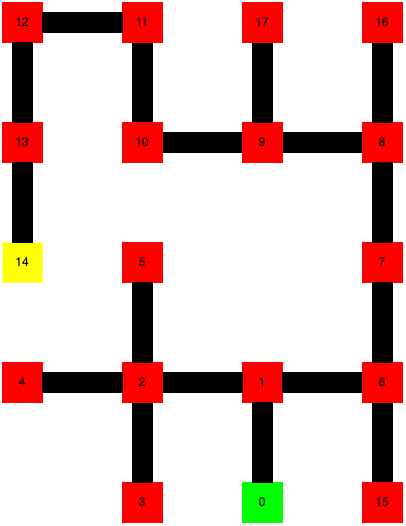
\includegraphics[scale=0.6]{resources/maze.png}
    \caption{Visual representation of the test maze}
    \label{fig:maze}
\end{figure}

The maze comprises 15 squares connected by straight lines that the robot must follow. The green square in Figure \ref{fig:maze}, represents the start of the maze and the yellow square marks the end. The maze was designed to contain at least one of all the intersection types described in Figure \ref{fig:intersection_types} and maintain an acceptable size.

To simplify the intersection scanning and manoeuvring process, only 90° turns are allowed; therefore, the maximum number of paths connected to one intersection is four. These criteria result in the eight intersection types represented in Figure \ref{fig:intersection_types}. Here the arrows show the path from which the robot approaches the intersection. The test maze represented in Figure \ref{fig:maze} contains all eight intersection types.

\begin{figure}
    \centering
    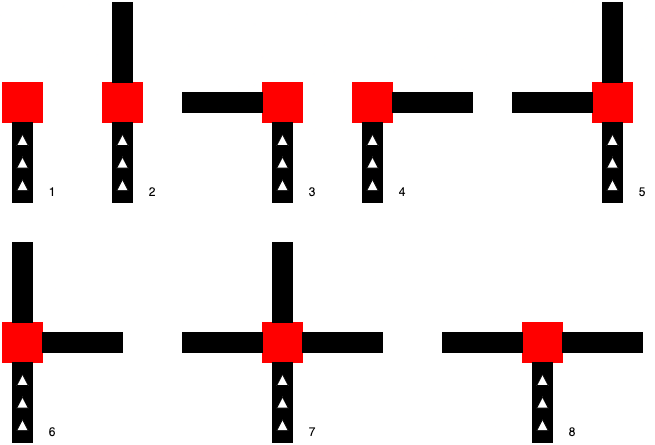
\includegraphics[width=\textwidth]{resources/intersectiontypes.png}
    \caption{Visual representation of the intersection types}
    \label{fig:intersection_types}
\end{figure}

All red squares (intersections) have a width of 6cm, and the black lines (paths) connecting them have a length of 12cm and a width of 1,8cm. The intersections are wider than the paths, so the robot does not miss them even if it does not approach the intersection perfectly aligned.
The length of the paths is optimised to keep the labyrinth as small as possible but, at the same time to give the robot enough space to align itself after an intersection. Different widths of the paths were tested, and it was found that the width of two parallel insulating tapes (1,8 cm) worked best. Too narrow paths cause the robot to overshoot the line during realignment, resulting in repeated attempts at realignment. Paths that are too wide cause the robot to arrive at an intersection at an oblique angle, resulting in incorrect intersection type detection.

In general, different colours have been used to make it possible to detect intersections start and finish of the maze with a single colour sensor. This is necessary for navigation and for taking time and energy measurements. The robot detects intersections because of their red colour. At the intersections, the robot performs an intersection scan described in Sections \ref{sec:fixed_intersection_scan} and \ref{sec:turning_intersection_scanning}, and the time it takes the robot to do this is measured.

To build the labyrinth, a white plastic sheet and coloured insulating tape were used. Both materials are slightly shiny, which is not ideal because of the occasional mismeasurements. For example, "blue" is sometimes measured when the sensor is at the edge of a path. Although the materials are not ideal, they are cheap and allow for quick customization of the maze.


\subsubsection{Robot configurations}
The following sections explain the different robot configurations used for the tests:
\begin{itemize}
    \item Fixed-sensor robot (\FixRob)
    \item Turning-sensor robot (\TurnRob)
\end{itemize}

\noindent The robot configurations were chosen to test whether a rotating color sensor is advantageous for line tracking and intersection scanning compared to a fixed sensor.

The part of the robot that provides propulsion, namely the two motorized front wheels and the rear steering wheel, remains the same for each configuration. This makes the robots more comparable and enables focused testing of the robots' sensor configuration. What changes between the robots is the sensor configuration for detecting the colour of the ground.

\begin{figure}[h!]
    \centering
    \subfloat[Front side]
    {\label{fig:robot_chassis:front}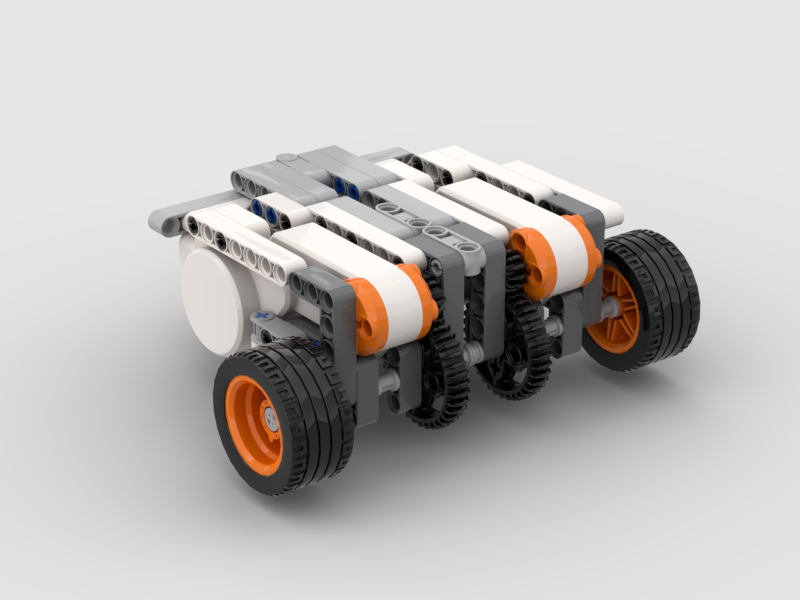
\includegraphics[width=.45\linewidth]{resources/nxt-render-front.png}}\hfill
    \subfloat[Back side]{\label{fig:robot_chassis:back}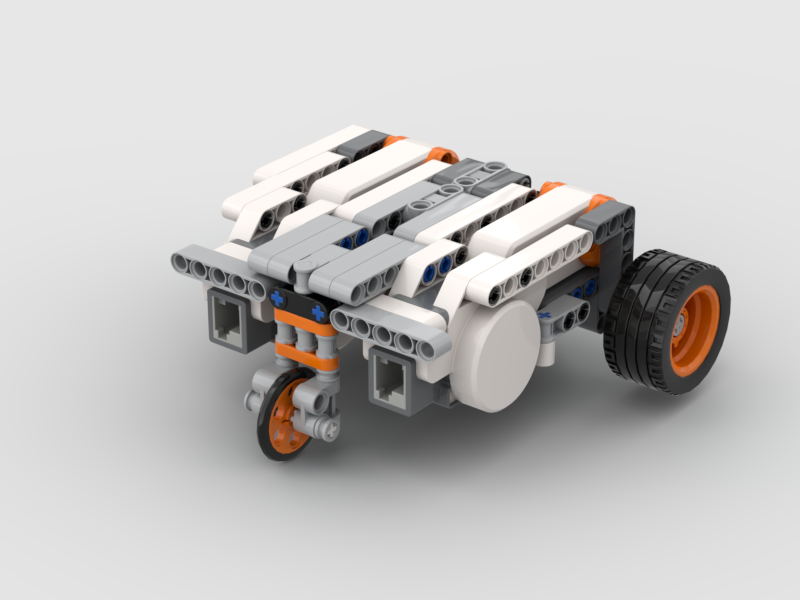
\includegraphics[width=.45\linewidth]{resources/nxt-render-back.png}}\par
    \subfloat[Drive wheel gears]{\label{fig:robot_chassis:gear}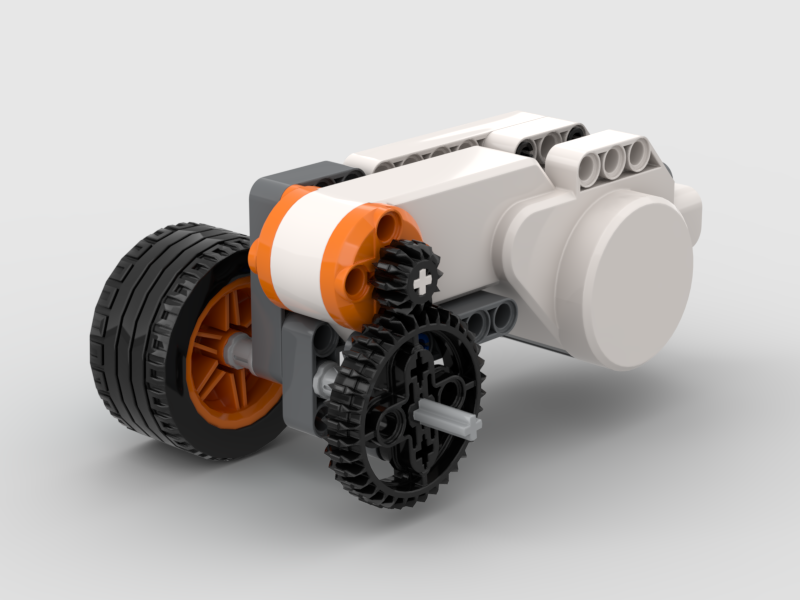
\includegraphics[width=.45\linewidth]{resources/nxt-render-drive-gear.png}}
    \caption{Render of robot chassis (Created in Bricklink Studio 2.0)}
    \label{fig:robot_chassis}
\end{figure}

All robots used for these tests were built from the LEGO Mindstorms NXT 2.0\footnote{\url{https://education.lego.com/en-us/downloads/retiredproducts/nxt/software}} kit and custom-designed for this task. The build instructions for the driving part of the robot can be found in the readme of the nxt\_ros2\footnote{\url{https://github.com/marvinknoll/nxt_ros2}} repository.

The robots have two drive wheels at the front, 13.5 cm apart, as visualised in Figure \ref{fig:robot_chassis:front}. Both are driven by an individual NXT motor, which enables differential drive. To increase the driving accuracy of the robot, a gear ratio of 3:1 between the motor and wheel was used (see Figure \ref{fig:robot_chassis:gear}). On the back of the robot is a non-driven, freely rotating castor wheel, which allows the robot to turn on the spot (see Figure \ref{fig:robot_chassis:back}).

\paragraph{Fixed-sensor robot (FixRob)}\label{sec:fixrob}

The \FixRob configuration consists of a single non-moving colour sensor. This sensor is mounted to scan the colour of the ground 9.5cm in front of the robot and is aligned with the robot's centre (see Figure \ref{fig:maze_solver:front}). The sensor is positioned approximately 2-3mm from the ground, which is the ideal distance according to the research of Pakdaman and Sanaatiyan \cite{pakdaman}.
This robot configuration does not use the motor to which the sensor is attached.

\begin{figure}[h]
    \centering
    \subfloat[Front side]{\label{fig:maze_solver:front}\includegraphics[width=.45\linewidth]{resources/nxt-img-front.jpg}}\hfill
    \subfloat[Back side]{\label{fig:maze_solver:back}\includegraphics[width=.45\linewidth]{resources/nxt-img-back.jpg}}
    \caption{Maze solving robot on the test maze}
    \label{fig:maze_solver}
\end{figure}

This robot configuration costs 110\euro\ considering only the electronic parts. The parts required are:
\begin{itemize}
    \item 1x NXT Brick - 60\euro
    \item 2x Motors - 15\euro
    \item 1x Colour sensor - 20\euro
\end{itemize}

\paragraph{Turning-sensor robot (TurnRob)}\label{sec:turnrob}

The \TurnRob configuration comprises one 180° turnable colour sensor. The sensor is attached to an NXT motor mounted on the robot (see Figure \ref{fig:maze_solver:front}). Turning the motor allows the sensor to rotate 90° in both directions. Since the NXT motors do not have an absolute encoder but only a relative encoder, the robot can't know the position of the motor/sensor but only the position relative to its starting point. Thus the sensor must be manually aligned with the centre of the robot before the execution. A 3:1 gearbox between the motor and the sensor improves rotation accuracy.

The idea behind this robot configuration is that only the sensor rotates at the intersection 
to check which paths are available. Once the scan is complete and the correct path is selected, the robot realigns itself and moves on. The detailed intersection scanning process is explained in Section \ref{sec:turning_intersection_scanning}.
The sensor does not turn for alignment on the track, but the robot rotates.

The cost for this robot configuration lies at 125\euro\ considering only the electronic parts. The parts required are:
\begin{itemize}
    \item 1x NXT Brick - 60\euro
    \item 3x Motors - 15\euro
    \item 1x Colour sensor - 20\euro
\end{itemize}

\subsubsection{Software setup}
\paragraph{General} \label{sec:software_setup_general}

The robots were programmed in Python using the Robot Operating System 2 (ROS2). The entire code runs on a host machine that needs to be constantly connected to the robot via a USB cable. The ROS2 package \textit{nxt\_ros2}\footnote{\label{fot:nxt_ros}\url{https://github.com/marvinknoll/nxt\_ros2}}, created by the author, was used to integrate the NXT brick into ROS2. The setup is visualised in Figure \ref{fig:sw_architecture}.

\begin{figure}[h]
    \centering
    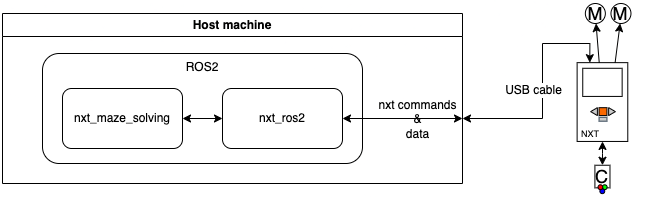
\includegraphics[width=\textwidth]{resources/architecture.png}
    \caption{General software architecture}
    \label{fig:sw_architecture}
\end{figure}

Although this setup has a slower feedback loop between the sensor input and motor output compared to running the code directly on the robot, it allows the use of the various tools provided by ROS2.

The code for making the robots follow lines and drive through the maze was put in a separate ROS2 package called \textit{nxt\_maze\_solving}\footnote{\url{https://github.com/marvinknoll/nxt_maze_solving}}. This package uses the ROS2 interfaces provided by \textit{nxt\_ros2}\footref{fot:nxt_ros} to receive sensor data and control the motors.

Detailed documentation of how \textit{nxt\_ros2} works internally can be found in its Readme file on GitHub\footref{fot:nxt_ros}.


\paragraph{Generic maze-solving algorithm}

To make the different robots more comparable, they use the same underlying generic algorithm described in Figure \ref{fig:generic_maze_solving_algorithm}; for navigating and solving the maze. The strategy to solve the maze is called “left-hand-rule”, where the robot always chooses the leftmost path at each intersection.

The robot initially sends a "Start" benchmarking message with the battery voltage and timestamp. It then enters a loop to find the end of the maze. In the loop, it uses sensor data to determine its state. If at an intersection, it scans the leftmost path and takes it. If it loses the line, it tries to align itself with it again. If on the line, it goes straight. If it reaches the end, it stops all motors and sends an "End" benchmarking message. Finally, statistics are calculated and stored before the program terminates.

\begin{figure}[hbt!]
    \centering
    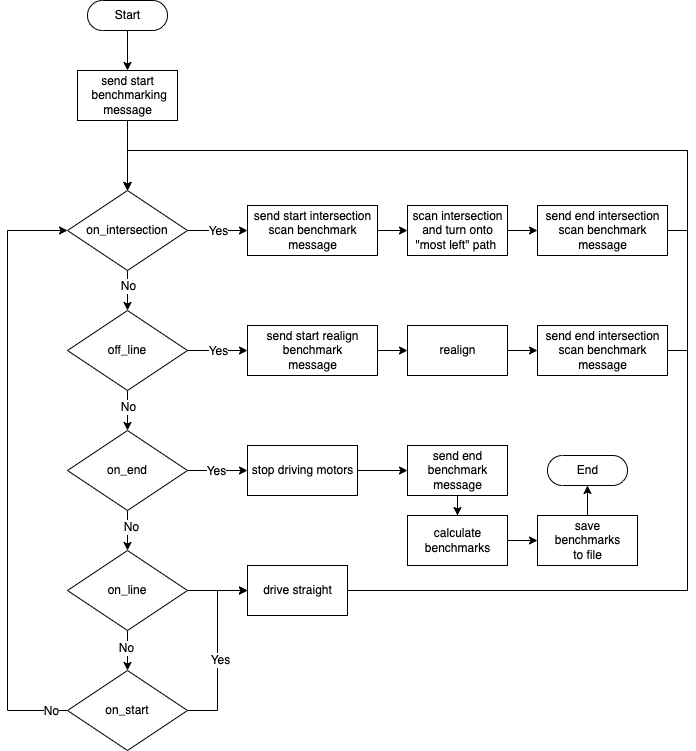
\includegraphics[width=\textwidth]{resources/generic-maze-solving-algorithm.png}
    \caption{Flowchart of the generic maze-solving algorithm}
    \label{fig:generic_maze_solving_algorithm}
\end{figure}

While the robots all follow the same maze-solving strategy, their methods for scanning intersections, realigning to the leftmost path and determining their states vary.

\clearpage

\paragraph{Fixed-sensor robot specific implementations}

Table \ref{tab:custom_state_fixed_robot} explains the specific implementations of the functions for determining the robot state.

\begin{table}[hbt!]
\caption{\FixedSensorRobot's custom state conditions}
\label{tab:custom_state_fixed_robot}
\centering
\begin{tabular}{l|p{\linewidth-4cm}}
\textbf{State}   & \textbf{Custom Implementation (Pseudo code)}                        \\ 
\hline
on\_line         & colour\_sensor\_value == black                                      \\
off\_line        & (colour\_sensor\_value == white) and (scanning\_intersection == False)    \\
on\_intersection & (colour\_sensor\_value == red)  \\
on\_start        & colour\_sensor\_value == green                                      \\
on\_end          & colour\_sensor\_value == yellow                                    
\end{tabular}

\end{table}

The intersection scanning and realignment strategies are implemented as state machines to keep the code more readable. For example, the intersection scan sequence was divided into several individual operations, each corresponding to a state machine's state.

\subparagraph{State machine for intersection scanning and navigation}\label{sec:fixed_intersection_scan}

First, the robot positions itself so its centre of rotation is in the middle of the intersection. In the next step, the robot rotates 135 degrees counterclockwise around its axis to ensure it is on the left of a possible left path. Finally, the robot rotates clockwise until it finds a path, which must be the one furthest to the left and, therefore, the path to take. The number of degrees by which the robot has turned can be used to determine which path has been taken. Now the robot is aligned with the path taken and ready to drive forward to the next intersection.
Figure \ref{fig:fixed_intersection_scan_state_machine} in the appendix shows a detailed diagram of this state machine.

\subparagraph{State machine for realignment on the line} \label{sec:realignment_strategy}

When the robot gets “off\_line”, it begins a realignment process using a state machine. This makes the robot turn on the spot in one direction and then the other to find the line. The robot uses two strategies to optimise this process. First, it turns only 20 degrees in both directions to quickly find the line and avoid turning in the wrong direction for too long. If it still does not find the line, it expands the search to 60 degrees in both directions. The second strategy is that the robot remembers which way it turned at the last intersection, allowing it to make an educated guess about which side of the line it is on when it misses it. This allows the robot to turn in the direction where it expects to find the line and find it more quickly.

\paragraph{Turning-sensor robot specific implementations}

This robot configuration uses the custom implementations described in Table \ref{tab:custom_state_turning_robot} to distinguish between the individual states.

\begin{table}[hbt!]
\caption{\TurningSensorRobot's custom state conditions}
\label{tab:custom_state_turning_robot}
\centering
\begin{tabular}{l|p{\linewidth-4cm}}
\textbf{State}   & \textbf{Custom Implementation (Pseudo code)}                        \\ 
\hline
on\_line         & colour\_sensor\_value == black                                         \\
off\_line        & (colour\_sensor\_value == white) and (scanning\_intersection == False) \\
on\_intersection & colour\_sensor\_value == red       \\
on\_start        & colour\_sensor\_value == green                                         \\
on\_end          & colour\_sensor\_value == yellow                                    
\end{tabular}

\end{table}

The intersection scanning and realignment strategies are again implemented using state machines. The realignment process for the \turningSensorRobot is the same as for the \fixedSensorRobot and is described in Section \ref{sec:realignment_strategy}.

\subparagraph{Strategy for intersection scanning and navigation} \label{sec:turning_intersection_scanning}

Once the robot is in the "on\_intersection" state, it repositions itself so that the colour sensor's centre of rotation is at the centre of the intersection (see Fig. \ref{fig:intersection_scan:init}). It then rotates the sensor 90 degrees counterclockwise (see Fig. \ref{fig:intersection_scan:left}). Next, it reads the sensor values while turning the sensor clockwise 135 degrees. If the robot detects the line during this process, it knows it has found the line. Depending on the angle of the line, the robot can determine whether the line represents the left or straight path. If the robot does not detect the line, it repositions the sensor at a 0-degree angle and then turns clockwise on the spot until it finds the right or back path.

\begin{figure}
    \centering
    \subfloat[Initial position]{\label{fig:intersection_scan:init}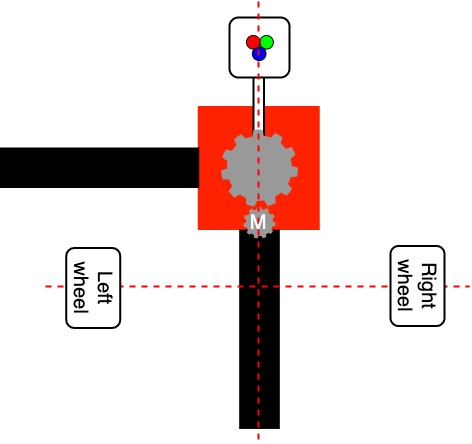
\includegraphics[width=.45\linewidth]{resources/intersection-scan-init.jpg}}\hfill
    \subfloat[Scan to the left]{\label{fig:intersection_scan:left}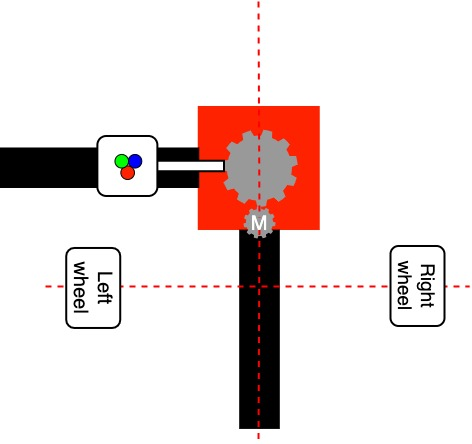
\includegraphics[width=.45\linewidth]{resources/intersection-scan-left.jpg}}
    \caption{Visual representation of \TurnRob's intersection scanning strategy}
    \label{fig:intersection_scan}
\end{figure}

This strategy avoids turning the robot in the wrong direction by scanning the left and straight path by turning only the sensor. A detailed diagram of this state machine can be found in the appendix in Figure \ref{fig:turning_intersection_scan_state_machine}. 

\subsection{Data collection} \label{sec:data_collection}

The data collection process included 11 test runs for each robot configuration, performed sequentially. The tests were conducted on November 18, 2022, for the \fixedSensorRobot and on November 22, 2022, for the \turningSensorRobot. The test maze was set up in a closed room, with the only light source being a conventional ceiling lamp.

The robot was powered by rechargeable nickel metal hydride (NiMH) batteries, which were fully charged and allowed to cool to room temperature before each test sequence. The charging and plugging order was the same for each test. The room temperature was maintained at 19-20°C for each robot configuration and test run.

Several measurements were taken during each test run. These included the total duration of the run, the start and end battery voltage in millivolts, and the duration of each intersection scan and realignment. Also counted were the number of realignments and whether the run was completed successfully or the robot failed to reach the end of the maze.

The decrease in battery voltage was calculated using the average voltage measurement taken at the start and end of each test. Both the start and end voltages were determined by taking 20 consecutive measurements and calculating the average of those readings. The data was collected, processed and then saved to a file using the measurement feature of the \textit{nxt\_maze\_solving} package and analysed in Google Sheets.

Since LEGO stopped selling some of the parts used in the robots, an average of the prices on eBay was calculated to estimate the cost of the robots.

The data collection method used allowed for accurate and reliable results. The controlled conditions ensured the data remained comparable and reproducible across all test runs. This allowed effective evaluation of the robot's performance.